\documentclass[12pt]{article}

\usepackage{sbc-template}

\usepackage{graphicx,url}

\usepackage[brazil]{babel}
\usepackage[latin1]{inputenc}

\sloppy

\title{TRUE: um sistema para rastreamento, localiza��o e identifica��o de usu�rios em ambientes inteligentes}

\author{Tales M. A. Porto\inst{1}, Danilo �. M. C. Ferreira\inst{1}, \\ Fabricio
N. Buzeto\inst{1}, Carla D. Castanho\inst{1}, Ricardo P. Jacobi\inst{1}}

\address{
Departamento de Computa��o -- Universidade Federal de Bras�lia (UnB)
}

\begin{document}

\maketitle

\begin{abstract}

Ubiquitous computing, or ubicomp, proposes that the computer should be something
invisible, helping and requiring minimal effort. For this invisibility becomes
real context sensitive applications should act proactively in the environment.
The System TRUE (Tracking and Recognizing Users in the Environment) makes the
identification, location and tracking of users in an intelligent environment and
 makes this information available to applications through the
middleware uos. We show here as the solution was constructed and their
experimental results.

\end{abstract}

\begin{resumo}

A Computacao Ub�qua, ou ubicomp, prop�e que a computa��o deveria ser algo
invis�vel, nos servindo e exigindo o m�nimo de esfor�o poss�vel. Para que essa
invisibilidade se torne real aplica��es sens�veis ao contexto devem atuar de
forma proativa no ambiente. O Sistema TRUE (\textit{Tracking and Recognizing
Users in the Environment}) realiza a identifica��o, localiza��o e rastreamento
de usu�rios em um ambiente inteligente e disponibiliza essas informa��es a
aplica��es atrav�s do middleware \textit{uos}. Mostraremos aqui como a solu��o
foi constru�da e seus resultados experimentais.

\end{resumo}

\section{Introdu��o}

Dentre as tecnologias envolvidas na cria��o de espa�os inteligentes, baseados 
nos conceitos de Computa��o Ub�qua ou Pervasiva ~\cite{weiser1, weiser2},
a sensibilidade ao contexto certamente representa um papel fundamental. 
A transpar�ncia no atendimento de demandas de um usu�rio requer informa��es
sobre ele, tais como identidade, localiza��o, estado f�sico e emocional e proximidade
de dispositivos dispon�veis no ambiente. Estabelecendo uma correla��o entre 
estas informa��es e servi�os solicitados, aplica��es inteligentes podem ent�o
auxili�-lo de forma mais eficiente.

% Seu enfoque est� em que a computa��o deveria ser algo
%invis�vel, nos servindo e exigindo o m�nimo de esfor�o poss�vel. 
%Permitindo assim, que o usu�rio tenha mais foco na tarefa em execu��o
%que na ferramenta. Um ambiente com tais caracter�sticas � chamado de inteligente
%(\textit{smart space}) pois busca auxiliar seus usu�rios de modo proativo e
%transparente.

%A intelig�ncia esperada nestes ambientes � fruto de aplica��es que processam
%dados fornecidos pelos diversos dispositivos presentes, bem como coordenam suas
%a��es. Tendo em vista a dinamicidade do \textit{smart space}, uma vasta gama de 
%informa��es podem ser ser necess�rias para se construir o contexto. De maneira especial,
%podemos considerar como informa��es fundamentais a identifica��o e localiza��o do usu�rio. 
%De posse destas � poss�vel personalizar as a��es a serem realizadas pelas aplica��es %inteligentes bem como direcion�-las aos locais corretos de atua��o.

Diversas tecnologias tem sido utilizadas para determina��o da identidade e localiza��o
de pessoas. Informa��es biom�tricas podem ser obtidas a partir do processamento de
imagens, sons e impress�es digitais, principalmente. Sistemas de localiza��o podem
basear-se em dispositivos de r�dio frequ�ncia (RFID, \emph{bluetooth}, \emph{wifi}, \emph{zigbee}, etc.), ac�sticos,
piezoel�tricos (press�o) ou por processamento de imagens. Do ponto de vista do usu�rio, 
um fator que fortalece a transpar�ncia � a n�o necessidade de realizar um processo espec�fico para identifica��o, como fornecer a impress�o digital ou focar uma c�mera para processamento da �ris, por
exemplo. 

V�rios aspectos devem ser considerados na sele��o das tecnologias para este prop�sito. Custo,
confiabilidade, grau de transpar�ncia e disponibilidade de dispositivos para sua implementa��o s�o
alguns aspectos principais. Em ambientes onde a aquisi��o de imagens � permitida, o seu processamento 
pode ser utilizado tanto para a identifica��o quanto para a localiza��o de pessoas. Por outro lado, o 
surgimento de dispositivos poderosos e de baixo custo nesta �rea, como o Kinect 
~\cite{kinect_microsoft}, torna-a uma alternativa interessante a ser considerada.
 
Nesse contexto, este artigo apresenta um sistema de rastreamento, localiza��o e 
identifica��o de usu�rios baseado em processamento de imagens, integrado a um 
\emph{middleware} que prov� servi�os para ambientes inteligentes. O sistema � 
denominado TRUE (\textit{Tracking and Recognizing User in the 
Environment}). TRUE obt�m informa��es do ambiente utilizando o sensor Kinect
~\cite{kinect_microsoft} da Microsoft e disponibiliza seus resultados para aplica��es 
sens�veis ao contexto atrav�s do \emph{Middleware} \textit{uOS}~\cite{fabriciobuzzeto2, fabriciobuzzeto}. 
O uOS incorpora uma infraestrutura de suporte a aplica��es sens�veis ao contexto
baseada em ontologias ~\cite{Ozaki2011}. A integra��o do sistema TRUE ao uOS 
viabiliza a constru��o de ontologias de localiza��o, entre outras. 
\section{Reconhecimento Facial e Rastreamento}

%Em ambientes inteligentes, as informa��es de contexto sobre os usu�rios como
%localiza��o e identidade s�o de grande import�ncia, proporcionando uma maior
%acur�cia nas tomadas de decis�es. A sua obten��o apresenta
%diversos desafios tendo em vista que os usu�rios se movimentam e
%interagem entre si e com os dispositivos de forma din�mica.

% -----

Dentre as diversas formas de se identificar um usu�rio, incluindo reconhecimento da �ris e  
de voz, o reconhecimento por meio da face se destaca devido a sua aquisi��o ser
realizada de maneira n�o intrusiva. Por�m,  o reconhecimento desta informa��o
apresenta desafios devido a varia��es de ilumina��o, �ngulos e poses,
express�es e maquiagem, dentre outros. Neste cen�rio, o processo de
reconhecimento facial pode ser divido em duas tarefas principais: a detec��o das
faces nas imagens e o reconhecimento destas.

A detec��o de faces � definida como o processo que determina a exist�ncia, ou
n�o, de uma ou mais faces em uma imagem. Atualmente existem diferentes m�todos
para realizar esta tarefa. Dentre eles se destaca o
\textit{Viola-Jones}~\cite{edsonma, violajones}, que � largamente utilizado. Tal
m�todo pode ser utilizado para construir uma abordagem de detec��o facial de
maneira r�pida e eficaz utilizando apenas imagens em tons de cinza, o que o
distingue dos outros m�todos, al�m do mesmo obter altas taxas de acerto.

Para o reconhecimento, busca-se padr�es nas faces de forma que estes possam ser
usados para a identifica��o do usu�rio. A t�cnica \emph{Eigenfaces}~\cite{hewitt}
consiste em extrair as principais caracter�sticas de uma face e, com base nelas, �
determinado um valor correspondente, o \textit{eigenvalue}. Para tanto � aplicada
a t�cnica de PCA (\textit{Principal Component Analisys})~\cite{belhumeur} em
imagens conhecidas. Com isto se obt�m um valor de \textit{eigenvalue} m�dio bem
como a dist�ncia de cada face para este valor. Assim quando se identifica uma
nova face, se calcula o valor do \textit{eigenvalue} e se compara com as
dist�ncias conhecidas. Esta t�cnica apresenta bons resultados sendo amplamente
utilizada em diversas bibliotecas, como a OpenCV~\cite{opencv_library}.

% -----

Para a localiza��o do usu�rio podemos utilizar a t�cnica de imagens de
profundidade onde a cada pixel da imagem � atrelado a um valor de dist�ncia
relativa ao sensor. Dentre as t�cnicas conhecidas destacam-se TOF
(\textit{Time of Flight})~\cite{jain, fall-detection} e luz
estruturada~\cite{fall-detection}. Uma imagem de profundidade n�o pode ser
obtida utilizando somente um sensor de v�deo. Por�m, adicionando uma textura
artificial na cena, uma imagem de profundidade pode ser recuperada. Esse
princ�pio consiste na proje��o de pontos de luz infravermelhos na cena que s�o
recuperados por uma c�mera infravermelha que l� a textura. Trata-se de um m�todo
mais acess�vel que o TOF, por�m pouco eficiente para estimar a dist�ncia nas
bordas dos objetos e em posi��es muito longe do sensor.

% -----

O rastreamento pode ser definido como o problema de estimar a trajet�ria de uma
entidade (objeto ou pessoa) em um plano de imagem a medida que se move na
cena. Em um ambiente inteligente, o rastreamento de pessoas � uma das principais
ferramentas para detectar novos usu�rios e serve como base para que novas
informa��es possam ser coletadas~\cite{yilmaz}. Basicamente, o processo de
rastreamento pode ser dividido em duas etapas: detec��o do objeto e rastreamento
do objeto detectado. Existe um forte relacionamento entre as t�cnicas de
rastreamento e a representa��o usada pelas mesmas. Dentre as representa��es
conhecidas destacam-se: por pontos; por formas geom�tricas primitivas; por
silhueta e contorno; por modelos de formas articuladas e por modelos de
esqueletos. A representa��o por silhueta e contorno � mais indicada para
rastrear entidades complexas de forma n�o r�gida. Ela � popular devido a sua
simplicidade, sendo muito utilizada no rastreamento de pessoas.

Todo m�todo de rastreamento requer um mecanismo de detec��o que
pode ser realizado a cada \textit{frame} (quadro) obtido ou na primeira vez que
a entidade a ser rastreada entra no campo de vis�o. Dentre os m�todos de
rastreamento se destacam o detector de pontos, a subtra��o de fundo e
a segmenta��o. A subtra��o de fundo � um m�todo popular para segmenta��o de
movimento, especialmente nas situa��es em que o plano de fundo � relativamente
est�tico. Ele detecta as regi�es de movimento na imagem obtendo a diferen�a
pixel a pixel entre o quadro corrente e o quadro referente ao plano de fundo.

Os m�todos de rastreamento de entidades mais utilizados atualmente s�o o
rastreamento de pontos, o rastreamento de n�cleo e o rastreamento de silhuetas.
O rastreamento de silhuetas � feito estimando a regi�o da entidade a cada
quadro a partir das silhuetas geradas nos quadros anteriores. Dado os modelos
de entidades, silhuetas s�o rastreadas por qualquer forma de correspond�ncia ou
evolu��o de contorno.
\section{Trabalhos Correlatos}
	
Rastreamento, localiza��o e identifica��o de usu�rios � um tema que tem motivado
diversos trabalhos na academia. A seguir s�o apresentados alguns projetos que se
destacam dentro desta �rea de pesquisa.

O Projeto CHIL \cite{chil, computerschil} possui foco em auxiliar nas intera��es
de pessoas em ambientes colaborativos, como salas de reuni�es e palestras. Ele
utiliza dados de �udio e v�deo do ambiente como fontes de informa��o.
Por�m, para a identifica��o e localiza��o dos usu�rios � utilizado apenas o
�udio coletado atrav�s de um vetor de microfones.

O \textit{SmartFlow} \cite{salah} � um \emph{middleware} que realiza a detec��o de
movimento, o rastreamento de pessoas, o reconhecimento facial e a localiza��o baseada em �udio.
O objetivo do sistema � identificar cada usu�rio ao entrar pela porta e
rastre�-lo no ambiente. Para identificar os usu�rios no momento da entrada o ambiente
possui uma c�mera voltada para a porta que fornece imagens de qualidade superior.

O AVIARY e MICASA~\cite{trivedi} s�o dois \textit{smart spaces}. Estes
ambientes inteligentes s�o separados fisicamente, por�m conectados. O primeiro
(AVIARY) foi projetado para ser uma pequena sala de confer�ncias e o segundo
(MICASA) uma pequena sala de aula. Nesse trabalho foi
desenvolvida uma nova arquitetura para ambientes inteligentes chamado DIVA. O
sistema proposto monitora o ambiente em baixa resolu��o de
forma cont�nua, detectando somente presen�a e dimens�es da entidade detectada. Formas de
aquisi��o de imagens mais detalhadas s�o ativadas quando um evento ou atividade
de potencial interesse � detectado. Esses eventos s�o os focos de aten��o do
sistema.

Os projetos apresentados acima mostram avan�os na localiza��o e identifica��o de
usu�rios. Cada um busca utilizar os dados mais importantes ou abundantes
encontrados para estas finalidades (nos casos citados: �udio ou v�deo).
Entretanto, nestes o rastreamento � perdido quando da interrup��o do processo de identifica��o 
(a face do usu�rio n�o est� voltada  para a c�mera ou o usu�rio n�o est� falando). 

Estabelecer uma
correla��o com dados dispon�veis para manter o rastreamento do usu�rio, mesmo
durante momentos de oclus�o de sua identifica��o, � o foco do sistema TRUE.

\section{Sistema TRUE}

O sistema TRUE (\textit{Tracking and Recognizing Users in the Environment})
realiza a identifica��o, localiza��o e rastreamento de usu�rio em um ambiente
inteligente. Para isso s�o utilizados os dados de v�deo e profundidade providos pelo sensor
\textit{Kinect}~\cite{kinect_microsoft}. Por fim estas informa��es s�o disponibilizadas
para as aplica��es atrav�s do middleware \textit{uOS}~\cite{fabriciobuzzeto, alegomes}.
O projeto � composto por 4 m�dulos conforme representado na
Figura~\ref{fig:relacao-modulos}.

\begin{figure}[htb]
	\begin{center}
		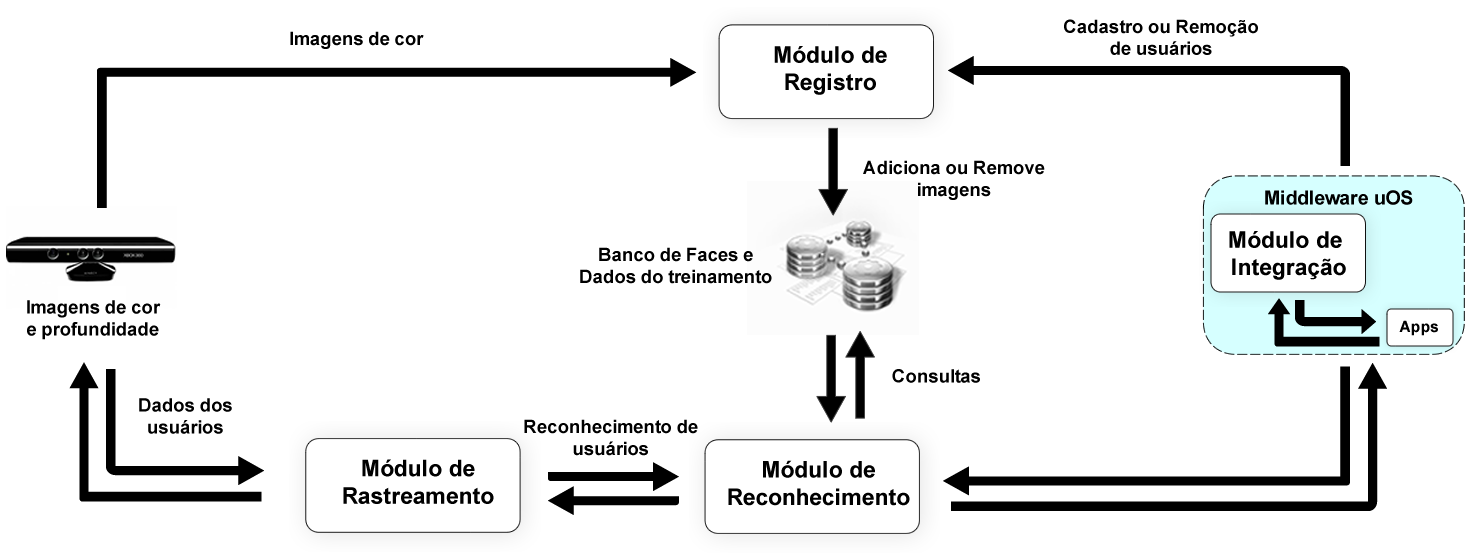
\includegraphics[scale=0.5]{img/modulo-integracao.png}
	\end{center}
	\caption{Intera��o entre o m�dulos do Sistema TRUE.}
	\label{fig:relacao-modulos}
\end{figure}

\subsection{M�dulo de Rastreamento}

O M�dulo de Rastreamento � respons�vel por rastrear os usu�rios no ambiente,
determinar a sua localiza��o f�sica em rela��o ao sensor \textit{Kinect} e
gerenciar suas identidades. Para realizar o rastreamento e localiza��o dos
usu�rios � utilizada a biblioteca \textit{OpenNI} (\textit{Open Natural
Interaction}). Trata-se de um \textit{framework} que define \textit{APIs} para o
desenvolvimento de aplica��es de intera��o natural.

Para a detec��o e rastreamento do usu�rio � utilizada a t�cnica de subtra��o de
fundo com a representa��o de silhuetas. A localiza��o, por sua vez, � realizada
utilizando-se imagens de profundidade que fornecem as coordenadas do centro de
massa do usu�rio. Tais coordenadas s�o compostas por tr�s dimens�es onde o
sensor � considerado como a origem do plano.

O processo de rastreamento come�a inicializando o dispositivo de entrada, no
caso o sensor \textit{Kinect}, registrando as a��es a serem tomadas quando
eventos em rela��o aos usu�rios ocorram, como, por exemplo, evento de novo
usu�rio detectado ou usu�rio perdido. Obt�m-se ent�o uma imagem de fundo da cena
que ser� utilizada no processo de subtra��o de fundo. Para cada imagem obtida da
cena, o processo de subtra��o de fundo � realizado atualizando os par�metros de
cada usu�rio, como sua posi��o na imagem e sua posi��o em rela��o ao sensor.

O M�dulo de Rastreamento det�m as informa��es sobre todos os usu�rios rastreados
no ambiente e � respons�vel por requisitar identifica��o ao M�dulo de
Reconhecimento. Isto acontece sempre que um novo usu�rio for detectado ou quando
for necess�rio reconhecer novamente um usu�rio j� rastreado. Quando um novo
usu�rio for detectado, o M�dulo de Rastreamento obt�m 20 imagens de cor
sucessivas deste usu�rio. De cada imagem � extra�da a regi�o correspondente a
face e enviada ao M�dulo de Reconhecimento requisitando identifica��o ao mesmo.
O M�dulo de Reconhecimento, por sua vez, realiza o reconhecimento facial e
retorna ao M�dulo de Rastreamento o nome do usu�rio e a confian�a obtida. A cada
500ms, o M�dulo de Reconhecimento verifica se chegou algum resultado de
identifica��o. Caso tenha chegado, o M�dulo de Rastreamento computa o resultado
e decide qual identidade ser� atribu�da ao respectivo usu�rio.

Ao inv�s de realizar o reconhecimento somente quando novos usu�rios s�o
detectados, com o objetivo de melhorar a confian�a do reconhecimento, o Sistema
TRUE realiza continuamente a identifica��o dos usu�rios j� reconhecidos. Essas
tentativas de reconhecer novamente os usu�rios ocorrer�o a cada 5 segundos
seguindo as mesmas etapas de quando um novo usu�rio for detectado. A �nica
etapa que se difere � a primeira, ou seja, ao inv�s de obter v�rias imagens de
um mesmo usu�rio, � obtida uma imagem de cada usu�rio rastreado e a mesma �
enviada ao M�dulo de Reconhecimento.

Ao obter um resultado de reconhecimento para determinado usu�rio, o M�dulo de
Rastreamento deve computar qual identidade ser� atribu�da ao mesmo. Para isso,
este m�dulo mant�m para cada usu�rio o n�mero total de vezes que este j� foi
reconhecido e os diferentes nomes obtidos pelo M�dulo de Reconhecimento bem
como a confian�a m�dia para cada nome e o n�mero de vezes que cada nome foi
atribu�do �quele usu�rio. Com todos esses dados, a identidade do usu�rio �
definida por meio da F�rmula~\ref{eq:media_ponderada}.

\begin{equation}
	\label{eq:media_ponderada}
	M_p = \frac{N_1 * C_1 + N_2 * C_2 + ... + N_n * C_n}{N_1 + N_2 + ... + N_n}
\end{equation}

\subsection{M�dulo de Reconhecimento}
O M�dulo de Reconhecimento � respons�vel pela identifica��o dos usu�rios no
ambiente. Para isto � utilizada a imagem do usu�rio (obtida pelo m�dulo de
rastreamento) de onde se obt�m a face do mesmo. Desta forma o reconhecimento
pode ser realizado sem atua��o expl�cita ou intrus�o nas atividades do usu�rio.
Seu funcionamento consiste nos seguintes passos:

\begin{enumerate}
	\item Obten��o da imagem de entrada composta somente pelo usu�rio cujo
	 reconhecimento foi requisitado. 
	\item Pr�-processamento da imagem, ou seja, convers�o da imagem em escala de
	cinza.
	\item  Detec��o facial na imagem. Caso nenhuma face seja encontrada, retorna
	 ``vazio''. Observa-se que no m�ximo uma face pode ser encontrada nesta
	 imagem.
	\item  Processamento da imagem, ou seja, uma nova imagem � criada recortando a
	regi�o da face encontrada. A imagem �, ent�o, redimensionada e equalizada criando assim
	um padr�o de tamanho, brilho e contraste aumentando a acur�cia do reconhecimento.
	\item  Reconhecimento facial com a t�cnica Eigenfaces. 
	\item  Retorno do nome do usu�rio com a face ``mais parecida'' e a confian�a do
	 reconhecimento.
\end{enumerate}

A detec��o facial foi desenvolvida utilizando o m�todo
\textit{Viola-Jones}~\cite{edsonma, violajones}. O \textit{Viola-Jones} �
implementado pela biblioteca \textit{OpenCV}~\cite{opencv_library} (\textit{Open
Source Computer Vision}). Basicamente, o processo de detec��o facial procura por
uma face em uma imagem pr�-processada. Para realizar detec��o facial utilizando
o m�todo \textit{Viola-Jones} � necess�rio a utiliza��o de um classificador em
cascata. O Sistema TRUE utiliza um classificador treinado para detectar faces
frontais em imagens.

O reconhecimento facial foi desenvolvido utilizando a t�cnica
\textit{Eigenfaces}~\cite{hewitt, artigo-eigenface}. Consiste em uma t�cnica
bastante satisfat�ria quando utilizada sobre uma base de faces relativamente
grande, permitindo ao sistema inferir, das imagens das faces suas principais
caracter�sticas e, partindo delas, realizar o reconhecimento facial utilizando
um n�mero reduzido de c�lculos, permitindo, assim, um reconhecimento em tempo
real. A base de dados utilizada no Sistema TRUE � formada por imagens no formato
PGM (\textit{Portable Gray Map}) com tamanho de 92x112 pixels e em escala de
cinza.

O reconhecimento facial inicia-se projetando a imagem no subespa�o atrav�s do
m�todo PCA~\cite{belhumeur} que reduz sua dimensionalidade. Ent�o, calcula-se a
dist�ncia da imagem projetada a cada um dos \textit{eigenfaces} obtidos na etapa
de treinamento obtendo uma lista de dist�ncias. Esta lista de dist�ncias �
comparada com a lista de dist�ncias de cada usu�rio, tamb�m obtidas na etapa de
treinamento, obtendo o usu�rio cuja lista de dist�ncias � a mais similar. Para o
c�lculo da dist�ncia � utilizado tanto a dist�ncia Euclidiana como o Mahalanobis
~\cite{perlibakas}. Conforme exposto na Sess�o \ref{sec:testes} foi observado
que a utiliza��o de ambas apresentou resultados mais satisfat�rios que ambas
isoladamente.

\subsection{M�dulo de Registro}

O M�dulo de Registro � respons�vel por cadastrar novos usu�rios no sistema e
trein�-lo para tamb�m reconhecer esse novo usu�rio. Este consiste das seguintes
etapas:
\begin{enumerate}
	\item Obten��o das imagens do novo usu�rio;
	\item Processamento das imagens, isto �, as imagens s�o convertidas em escala
	 de cinza, novas imagens s�o criadas recortando a regi�o da face encontrada.
	 Em seguida, as imagens s�o redimensionadas e equalizadas criando assim
	 padr�es de tamanho, brilho e contraste;
	\item Armazenamento das imagens;
	\item Treinamento do sistema para reconhecer esse usu�rio.
\end{enumerate}

A �ltima etapa do m�dulo de registro consiste no treinamento do sistema. O
treinamento inicia-se liberando os atuais dados de treinamento. Ent�o, um vetor
de imagens � obtido lendo todas as imagens contidas no banco de faces. Atrav�s
deste vetor, obt�m-se a \textit{eigenface} m�dia, os \textit{eigenfaces} e os
\textit{eigenvalues}. Para cada usu�rio cadastrado no Sistema TRUE, suas imagens
s�o projetadas no subespa�o atrav�s do m�todo PCA  que reduz suas
dimensionalidades, e s�o calculadas suas dist�ncias em rela��o aos eigenfaces
obtendo um vetor de dist�ncias. Os \textit{eigenfaces}, os \textit{eigenvalues},
a \textit{eigenface} m�dia e os vetores de dist�ncias s�o armazenados e podem
ser utilizados pelo M�dulo de Reconhecimento.

Ap�s o treinamento, o Sistema TRUE � reiniciado para que o reconhecimento seja
feito utilizando as novas imagens e informa��es obtidas com o treinamento.

\subsection{Modulo de Integra��o}

O M�dulo de Integra��o � respons�vel por disponibilizar ao ambiente os dados dos
usu�rios. Para isto o Sistema TRUE disponibiliza um \textit{Driver} de Usu�rio
(\textit{UserDriver}) para o middleware \textit{uOS}. Tal \textit{driver}
fornece os seguintes servi�os de consulta e eventos: 

\begin{itemize}
	\item Servi�os:
	\begin{itemize}
		\item Consultas as informa��es dos usu�rios no ambiente: atrav�s dessas
			consultas, as aplica��es tem acesso aos nomes, e-mails, posi��es correntes e
			confian�a do reconhecimento de todos os usu�rios presentes no ambiente; 
		\item Cadastro: as aplica��es podem cadastrar novos usu�rios fornecendo ao
			\textit{UserDriver} o nome, o e-mail e as imagens do novo usu�rio;
		\item Treino do sistema: ap�s cadastrar novos usu�rios as aplica��es podem
			retreinar o sistema para poder reconhecer o novo usu�rio cadastrado;
		\item Remo��o: as aplica��es podem remover usu�rios cadastrados fornecendo o
		e-mail do usu�rio.
	\end{itemize}

	\item Eventos:
	\begin{itemize}	 
		\item Novo Usu�rio: evento gerado assim que um novo usu�rio foi detectado pelo
		 Sistema TRUE. 
		\item Usu�rio Perdido: evento gerado assim que um usu�rio deixou de ser
		 rastreado pelo Sistema TRUE. 
		\item Atualiza��o dos dados do usu�rio: evento gerado a cada cinco segundos
		 atualizando os dados de todos os usu�rios rastreados.
	\end{itemize}
\end{itemize}
\section{Ambiente e Resultados Experimentais}
\label{sec:testes}

Com o intuito de verificar o desempenho do Sistema TRUE foram realizados uma
s�rie de testes abrangendo os dados de Rastreamento, Localiza��o e
Reconhecimento. Tais testes foram realizados no Laborat�rio LAICO (LAborat�rio
de Sistemas Integrados e COncorrentes) do Departamento de Ci�ncia da Computa��o da
Universidade de Bras�lia. O ambiente onde os mesmos foram realizados �
exemplificado pela Figura~\ref{fig:laico}.

\begin{figure}[htb]
	\begin{center}
		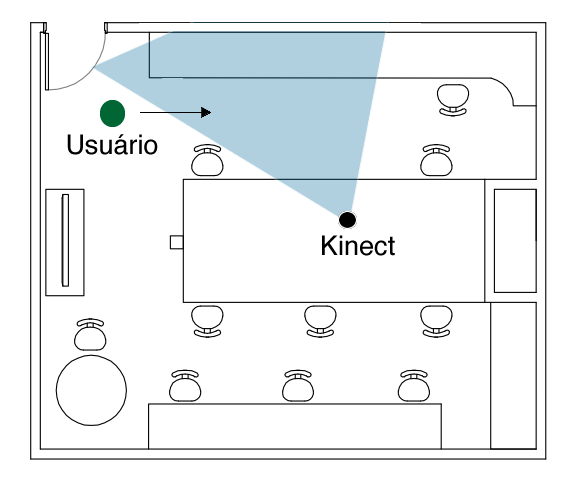
\includegraphics[scale=0.20]{img/laico-teste-deteccao.png}
	\end{center}
	\caption{Ambiente de testes.}
	\label{fig:laico}
\end{figure}

\subsection{Rastreamento}

Foram realizados testes com o objetivo de verificar a efici�ncia da detec��o e o
dimens�o da oclus�o dentro do sistema. A oclus�o era um problema esperado uma
vez que o Sistema TRUE utiliza somente um sensor \textit{Kinect} como
dispositivo de entrada. Os testes para a detec��o foram feitos simulando a
entrada de um usu�rio na cena e analisando o momento em que o mesmo era
detectado. Em todos os testes o usu�rio era detectado antes mesmo de entrar na
�rea de vis�o do sistema por completo.

Foram realizados dois testes para a oclus�o. No primeiro foi testado o caso em que
um usu�rio oculta propositalmente outro j� rastreado. Nesta situa��o, caso o
usu�rio rastreado continuasse oculto, o sistema o determinava como perdido. Por
outro lado, nos casos de oclus�o parcial, o sistema se mostrou robusto. No
segundo teste foi simulada a situa��o de oclus�o moment�nea, ou seja, um usu�rio
em movimento oculta outro por um curto per�odo de tempo em raz�o da sua
movimenta��o. Nestes casos, o sistema TRUE perde o usu�rio rastreado, mas
rapidamente � capaz de detect�-lo novamente.

Durante os testes realizados com rastreamento foi observado alguns problemas
quando o usu�rio rastreado interagia com objetos do ambiente ou com outros
usu�rios. Na grande maioria das vezes em que o usu�rio interagiu com objetos, o
Sistema TRUE considerou o objeto como sendo parte do usu�rio. Entretanto, esta
situa��o n�o prejudicou a efici�ncia do sistema. Por outro lado, os problemas
com intera��o entre usu�rios foram mais raros, por�m tiveram impacto maior. Tais
problemas consistem em ``interfer�ncias'' que ocorreram em algumas situa��es de
contato entre dois ou mais usu�rios. Apesar dos problemas relatados, o rastreamento conseguiu, na maioria dos testes,
atender �s necessidades rastreando os diversos usu�rios no ambiente em suas
atividades di�rias.

\subsection{Localiza��o}

O Sistema TRUE obt�m a localiza��o dos usu�rios no ambiente por meio de
coordenadas dos mesmos em rela��o ao \textit{Kinect}. Para verificar a acur�cia
dessas coordenadas foram realizados alguns testes. Os testes foram realizados
para as coordenada do eixo x e z.

Para testar a precis�o as coordenadas do eixo z foi realizado o seguinte teste:
um objeto (uma caixa de papel�o) foi colocada em frente ao sensor a diferentes
dist�ncias do mesmo (1000mm, 2000mm, 3000mm, 4000mm, 4057mm). Foi observado, a
discrep�ncia aumenta conforme o objeto se distancia do sensor. Neste teste o
menor erro obtido foi de 3,21mm e o maior de 111,75mm. Desta forma o sistema
apresenta um erro m�ximo de 3\% sobre os valores obtidos. Um valor que pode ser
considerado desprez�vel para a maior parte das aplica��es.

Para testar a precis�o das coordenadas do eixo x foi realizado o seguinte teste:
um objeto (uma caixa de papel�o) foi colocada a uma dist�ncia fixa de 3000
mil�metros do sensor e colocada em diferentes posi��es ao longo do eixo
$\displaystyle x$ (0, $\displaystyle \pm330mm$, $\displaystyle \pm660mm$,
$\displaystyle \pm990mm$). Foi observado que existe uma diferen�a constante de
poucos cent�metros ao longo de todo teste. � poss�vel inferir ent�o, a partir
dos dados obtidos, que o Sistema TRUE consegue fazer estimativas das coordenadas
no eixo $\displaystyle x$ com erro de poucos cent�metros. Neste caso o menor e
o maior erro obtido foi de 27,19mm e 79,29mm respectivamente. Chegamos ent�o a
um erro m�ximo de 10\% sobre os valores obtidos. Este � um valor mais
significativo que o teste anterior mas, ainda assim, pode ser relevado na maior
parte das aplica��es.

\subsection{Identifica��o}

Para testar os resultados de identifica��o foram realizadas 2 itera��es de
testes, uma vez que a primeira itera��o n�o apresentou resultados satisfat�rios.
Para an�lise foram utilizados tr�s percentuais: verdadeiro positivo, quando o
sistema identifica o usu�rio de maneira correta; verdadeiro negativo, quando o
sistema identifica o usu�rio de maneira errada; e falso negativo, quando o
sistema n�o identifica o usu�rio cadastrado.

No primeiro cen�rio de testes, os cadastros foram feitos utilizando
10 imagens de faces de cada usu�rio: 6 imagens frontais, 2 imagens da
face ligeiramente rotacionada para a direita e 2 imagens dela ligeiramente
rotacionada para a esquerda.  Essa estrat�gia tem
com o objetivo diminuir o impacto das varia��es de poses e �ngulo no
reconhecimento facial.  Observou-se que a taxa de Verdadeiro Positivo,
\textbf{73,63\%}, foi uma taxa baixa para um sistema de reconhecimento
autom�tico. A taxa de Verdadeiro Negativo,
\textbf{15,83\%}, foi bem superior a taxa de Falso Negativo, \textbf{8,34\%},
mostrando que a principal defici�ncia do reconhecimento facial consiste na
confus�o entre os usu�rios cadastrados no sistema.

Esses resultados n�o foram considerados satisfat�rios. Sob a hip�tese
do resultado ter sido influenciado pela baixa quantidade de faces e poses,
construiu-se um segundo cen�rio de testes, onde os cadastros foram feitos utilizando 100
imagens das faces de cada usu�rio em diferentes �ngulos, posi��es e express�es
faciais. No momento do cadastro, foi solicitado que os usu�rios movimentassem o
rosto levemente para cima, para baixo, para esquerda e para direita de maneira
aleat�ria e com diferentes express�es faciais.

Para esse segundo cen�rio houve um aumento na taxa de Verdadeiro Positivo de
\textbf{73,63\%} para \textbf{82,5\%} e redu��o significativa na taxa de
Verdadeiro Negativo de \textbf{15,83\%} para \textbf{5,46\%}, mostrando que os
casos de confus�es entre os usu�rios foram mais raros. A melhora obtida comprova
a hip�tese que um n�mero maior de poses e faces aprimorou a capacidade do
sistema de reconhecer seus usu�rios. Com uma maior variabilidade nos dados de um
mesmo usu�rio temos um melhor treinamento do sistema. Isso torna os valores de
\textit{eigenfaces} calculados mais robustos para uma maior diversidade de poses
a serem encontradas durante a execu��o.  

% \subsection{Integra��o}
% 
% Com intuito de exemplificar a utiliza��o do \textit{UserDriver} e testar a
% integra��o do Sistema TRUE com o middleware \textit{uOS} foi desenvolvido uma
% aplica��o para o middleware chamada \textit{UserApp}. Esta aplica��o registra um
% \textit{listener} para ``escutar'' os eventos do \textit{UserDriver} chamado
% \textit{UserListener}.
% 
% Quando o \textit{UserListener} � inicializado ele obt�m acesso ao Twitter e se
% registra para escutar os eventos gerados pelo \textit{UserDriver}. Para cada
% evento obtido, ele envia mensagens pelo Twitter para os usu�rios no ambiente.
% Para eventos de ``novo usu�rio detectado'' e ``usu�rio perdido'', ele envia
% mensagens de boas vindas e de despedidas respectivamente.  O
% \textit{UserDriver} tamb�m gera eventos de atualiza��o dos dados dos usu�rios.
% Quando estes eventos s�o gerados, o \textit{UserListener} verifica se houve
% atualiza��o na identidade do usu�rio e se o mesmo est� a mais de uma hora no
% mesmo lugar. Caso esteja, ele envia mensagens aos usu�rios informando estes
% acontecimentos.
% 
% Testes funcionais foram feitos com a aplica��o mostrando que o \textit{driver}
% consegue obter os dados �ntegros do Sistema TRUE e gerar os eventos de maneira
% praticamente instant�nea. A Figura mostra as mensagens geradas pela aplica��o em
% um teste funcional, onde Danilo, um usu�rio cadastrado, entra no ambiente senta
% em uma mesa com seu notebook permanecendo no mesmo lugar por mais de uma hora, e
% logo depois deixa o ambiente.
% 
% \begin{figure}[hbt]
% 	\begin{center}
% 		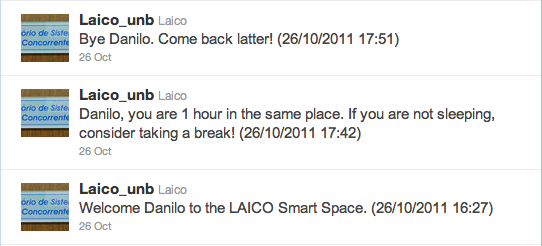
\includegraphics[scale=0.6]{img/tweets.png}
% 	\end{center}
% 	\caption{Exemplo das mensagens enviadas pelo Twitter aos usu�rios no ambiente.}
% 	\label{fig:tweets}
% \end{figure}


\section{Conclus�o}

Foram conduzidos conjuntos de testes para cada um dos prop�sitos do Sistema
TRUE. Os testes de rastreamento simularam diferentes situa��es di�rias onde os
usu�rios rastreados interagem entre si e com diferentes objetos. O Sistema TRUE
se mostrou eficaz tendo em vista que os novos usu�rios s�o detectados antes
mesmo de entrarem por completo no campo de vis�o do sensor. Al�m disso,
revelou-se robusto em casos de oclus�es parciais e como esperado, nos casos de
oclus�es totais n�o foi poss�vel prosseguir com o rastreamento. Os testes tamb�m
mostraram que os limites do sensor permitem at� 5 pessoas a uma dist�ncia de
4,057 metros.

Os testes de localiza��o foram realizados comparando as coordenadas obtidas pelo
Sistema TRUE com as coordenadas mensuradas manualmente. As coordenadas obtidas
pelo sistema se mostraram consideravelmente pr�ximas das reais, apresentando
diferen�as de poucos cent�metros que aumentam juntamente com a dist�ncia entre o
usu�rio e o sensor.

Foram realizados dois cen�rios de testes de identifica��o que se diferem na
estrat�gia utilizada no cadastro dos usu�rios. O segundo cen�rio utiliza uma
maior quantidade de imagens da face de cada usu�rio com uma maior varia��o dos
�ngulos, poses e express�es faciais. Os testes mostraram que a estrat�gia
utilizada no cadastro dos usu�rios tem grande impacto nos resultados do
reconhecimento, sendo que a taxa de acertos aumentou de 73,63\% (primeiro
cen�rio) para 82,5\% (segundo cen�rio).

Com as informa��es providas pelo Sistema TRUE, tornou-se poss�vel o
desenvolvimento de novas aplica��es que possuem um maior entendimento do
contexto do ambiente, como pode ser visto no \textit{UserApp}. Esta aplica��o
utiliza as identidades e posi��es dos usu�rios para enviar mensagens de boas
vindas, despedidas e mensagens para inform�-los a quanto tempo est�o no mesmo
lugar.

\subsection{Trabalhos Futuros}

Os dados providos pelo Sistema TRUE e disponibilizados pelo Middleware uOS
constroem uma nova base para a cria��o de in�meras aplica��es para ambientes
inteligentes. A partir das informa��es de identidade e localiza��o dos usu�rios,
tornou-se poss�vel desenvolver aplica��es de reconfigura��o autom�tica de
servi�os, estabelecimento de contextos e defini��o de perfis.

Al�m disso, o Sistema TRUE pode ser melhorado em algumas de suas
caracter�sticas. Uma dessas melhorias consiste na expans�o do sistema para
permitir a utiliza��o de m�ltiplos Kinects de modo a expandir sua �rea de
cobertura. Essa expans�o minimizaria os problemas de oclus�o e tamb�m aumentaria
o n�mero m�ximo de usu�rios rastreados.

� poss�vel tamb�m melhorar os resultados do reconhecimento. Como visto nos
testes, foi poss�vel obter melhores resultados apenas modificando a estrat�gia
de cadastro. Essa melhoria pode ser desenvolvida em duas frentes, como estudo de
novas formas de cadastros de usu�rio e novas t�cnicas que utilizam os dados de
profundidade para o reconhecimento facial.

\bibliographystyle{sbc}
\bibliography{bibliografia}

\end{document}
